\documentclass[10pt,conference,compsocconf]{IEEEtran}

\usepackage{hyperref}
\usepackage{amsmath}        % math
\usepackage{graphicx}   % For figure environment
\usepackage{todonotes}

\begin{document}
\title{Design of a Recommendation System using Ensembling}

\author{
  Luc\'{i}a Montero Sanchis, Nuno Miguel Mota Gon\c{c}alves, Matteo Yann Feo,  \\
  \textit{Department of Computer Science, EPFL Lausanne, Switzerland}
}

\maketitle

\begin{abstract}
  We evaluate the performance of  Collaborative Filtering methods for implementing a Recommendation System. With these methods we are able to obtain 0.9875 RMSE on a heldout test set. We consider both nearest neighbor methods and latent factor models for predicting new ratings. An ensemble predictor is built based on the previous methods employing Ridge Regression. The ensemble further reduces the RMSE to 0.9757 RMSE proving the validity of the approach.
\end{abstract}

\section{Introduction}
	The aim of this project is to implement a Recommendation System that predicts a numerical value $r_{ui}$ corresponding to the predicted rating of a user $u$ for an item $i$, based on the known past ratings for other users and items. The data provided consist on a first dataset of known user-item ratings (\emph{training}) and on a set of user-item pairs which rating values we need to predict (\emph{test}).

  Since the available data consists only on the past ratings without any information about the users or films, we focus on Collaborative Filtering (CF) techniques. Ensemble methods are one of the most successful approaches for this problem.

  We use an ensemble approach to combine the predictions obtained with well-known CF techniques, including neighborhood methods and latent factor models \cite{koren2009matrix}. This approach achieves better results when combining predictions that are very different from each other but achieve low RMSE scores individually, which is the reason why we use a variety of CF techniques. After adjusting the parameters of these predictors to minimize their individual RMSE, we use their predictions as features for Ridge Regression.

  One of the challenges we face is dealing with users and items that have a lower number of ratings, since some methods do not yield good results for these and are better at making predictions for items and users with a higher number of ratings.

\section{Models and methods}
	\label{sec:models-methods}
  We start by obtaining ratings predictions with each of the CF methods considered, that will be used as features when applying Ridge Regression for the ensembling.

  It is important to note that for the ensemble we will be training the Ridge Regression model on the predictions for the \emph{training} dataset, and then use the resulting weights to predict ratings for the \emph{test} dataset. In order to obtain better results we split the \emph{training} into 5 disjoint subsets with approximately the same number of entries. Then we obtain the predictions for each subset by training the models in the remaining 4 subsets. This assures that in the ensembling step more weight is given to the methods that obtain better results, which is important since when using ensembles it is not so essential that individual predictors have a very low RMSE \cite{toscher2009bigchaos}.

  We can further improve the results by increasing the number of features for Ridge Regression. We do this by defining \emph{meta-features} and afterwards building a polynomial basis of the features - which now include both the CF methods predictions and the meta-features.

  Lastly, we explain how we solved the problem of having a lower number of ratings for some users and items.

  \subsection{Collaborative Filtering (CF) methods} % (fold)
  \label{sub:collaborative_filtering_methods}
    In a first step we use several CF methods to obtain different predictions that we will later combine in the ensemble. We adjusted the parameters for each method using 5-fold cross-validation and grid-search.

    Afterwards we obtain the \emph{predictions} that we will use as features in the ensembling step. As explained previously, to obtain predictions for the \emph{training} dataset we divide it into 5 subsets, and for each one we generate the predictions by training on the remaining 4. When generating the predictions for the \emph{test} dataset we train the methods on the entire \emph{training} dataset.

    \subsubsection{Baseline} % (fold)
    \label{ssub:baseline}
      Much of the variation in the ratings is related to either users or items \cite{koren2009matrix}. One possible method for predicting values of ratings is shown in equation \ref{eq:bias}, where $\mu$ represents the global average rating, $b_i$ is the bias involved in rating $i$ and $b_u$ is the bias of user $u$.

      \begin{equation}
        \label{eq:bias}
        b_{ui} = \mu + b_i + b_u = \mu + \mu_i + \mu_u
      \end{equation}

      In our approach $b_i$ and $b_u$ are the average ratings per item and per user respectively, after subtracting $\mu$. This \emph{baseline} prediction ignores the interaction between users and items \cite{koren2009matrix}, but we still decided to consider it as a prediction method by itself.
    % subsubsection baseline (end)

    \subsubsection{Slope One} % (fold)
    \label{ssub:slope_one}
      Slope One algorithms propose a simple predictor function $f(x) = x + b$ to avoid overfitting. Equation \ref{eq:slope-one-1} shows the rating prediction $\hat{r}_{ui}$ for item $i$ by user $u$.

      \begin{equation}
          \label{eq:slope-one-1}
          \hat{r}_{ui} = \mu_u + \frac{1}{|R_i(u)|} \sum_{j \in R_i(u)} dev(i,j)
      \end{equation}

      Where $R_i(u)$ is the set of relevant items (items $j$ rated by $u$ with at least one common user with $i$) and $\text{dev}(i,j)$ is the average difference between the ratings of items $i$ and $j$ \cite{lemire2005slope}. We used the implementation of this algorithm provided in the Python Surprise library \cite{surprise}.

    % subsubsection slope_one (end)
    \subsubsection{K Nearest Neighbors (KNN)} % (fold)
    \label{ssub:k_nearest_neighbors}
      Neighboring methods base their predictions on the relationships between items or between users. The first item-oriented approach predicts a rating $\hat{r}_{ui}$ based on the known ratings of user $u$ for items \emph{similar} to $i$. Alternatively, the user-oriented approach predicts a rating $\hat{r}_{ui}$ based on the known ratings for $i$ by users with similar preferences to those of $u$ \cite{koren2009matrix, koren2010factor}.

      We used both approaches with the implementations provided in the Python Surprise library \cite{surprise} that take into account a baseline rating.

      \begin{itemize}
        \item {Item-based KNN} parameters (\texttt{KNN(i)}):
          \begin{itemize}
            \item k = 60
            \item min\_k = 20
            \item Similarity measure: Pearson baseline
          \end{itemize}
        \item {User-based KNN} parameters (\texttt{KNN(u)}):
          \begin{itemize}
            \item k = 300
            \item min\_k = 20
            \item Similarity measure: Pearson baseline
          \end{itemize}
      \end{itemize}
    % subsubsection k_nearest_neighbors (end)
    \subsubsection{Matrix Factorization (MF) methods} % (fold)
    \label{ssub:matrix_factorization_methods}
      As mentioned in the previous section, the baseline method (equation \ref{eq:bias}) does not take into account the interaction between users and items. This is why it is often used together with MF to predict ratings as shown in equation \ref{eq:mfbl}.
      \begin{equation}
        \label{eq:mfbl}
        \hat{r}_{ui} = b_{ui} + q_i^T p_u
      \end{equation}
      In this equation $q_i$ and $p_u$ are the factors that describe item $i$ and user $u$ respectively, and they are obtained by \emph{factorizing} the matrix that contains the known ratings.

      There are several approaches for MF in recommendation systems. One of them is Singular Value Decomposition (SVD), however its use is not recommended for sparse matrices since it is prone to overfitting. A similar approach includes a regularization term to avoid overfitting, as shown in equation \ref{eq:matrix-2}, and can be optimized using Stochastic Gradient Descent (SGD) or Alternating Least Squares (ALS) \cite{koren2009matrix}.

      \begin{equation}
        \label{eq:matrix-2}
        \min_{q*.p*} \sum_{(u,i) \in k} (r_{ui} - q_i^\top p_u)^2 + \lambda(||q_i||^2 + ||p_u||^2)
      \end{equation}

      The implementations we used for the project are the following:

      \begin{itemize}
        \item \emph{Truncated Singular Value Decomposition} (\texttt{SVD1})\\
          We used the approach from equations \ref{eq:mfbl} and \ref{eq:bias}. After subtracting the bias component, to obtain the item-user interaction we used the Truncated SVD implementation from the Scipy Python library \cite{scipy}. This function factorizes the entire sparse matrix (taking the zeros into account as well), so although the result can be computed analytically the number of features $k$ needs to be small. Otherwise for larger $k$ values the \emph{unknown} entries of the matrix will be predicted to be 0.

          The number of features we used is $k=13$.
        \item Singular Value Decomposition (\texttt{SVD2})\\
          We used the Python Surprise library \cite{surprise} implementation of SVD for sparse matrices including bias, that minimizes equation \ref{eq:matrix-2} using SGD methods.

          The parameters used are:
          \begin{itemize}
            \item biased: True
            \item k: 130
            \item reg\_all: 0.08
            \item n\_epochs: 50
          \end{itemize}

        \item Alternating Least Squares with Weighted Lambda Regularization (ALS-WR) (\texttt{ALS1})\\
          We used the ALS-WR implementation in Python from \cite{recommend}, which again minimizes equation \ref{eq:matrix-2}. The parameters used are:
          \begin{itemize}
            \item k: 20
            \item n\_iter: 50
            \item reg: 0.085
          \end{itemize}

        \item Alternating Least Squares implemented from scratch (\texttt{ALS2})\\
        We used the ALS algorithm that we implemented during the course, together with the baseline prediction from equation \ref{eq:bias}. Therefore, the prediction is done as shown in equation \ref{eq:mfbl}.

        However, since this algorithm takes a long time to converge to a solution we modified it slightly in order to allow the feature vectors to start from some given vectors (instead of starting from random values). These initial vectors (\texttt{u\_feats} and \texttt{i\_feats}) are the ones we obtained after the first iteration when training on the first of the fold \emph{training} dataset.

        The parameters we used are:
        \begin{itemize}
          \item k: 20
          \item lambda\_u: 0.1
          \item lambda\_i: 0.1
          \item tol: 1e-4
          \item max\_iter: 100
          \item init\_u\_features: u\_feats
          \item init\_i\_features: i\_feats
        \end{itemize}
        \item \emph{Non-negative Matrix Factorization} (\texttt{NMF})\\
          Non-negative Matrix Factorization is a MF technique where the user and item factors are kept non-negative. We have used the implementation provided in the Python Surprise library \cite{surprise}, where they apply stochastic descent with a step-size that ensures non-negativity as formally presented in \cite{zhang2006learning, luo2014efficient}.
          %\begin{equation}
              %\label{eq:nmf-1}
              %p_{uf}^{(t+1)} = p_{uf}^{(t)} \frac{\sum_{i \in I_u} q_{if} r_{ui}}{\sum_{i \in I_u} q_{if} \hat{r}_{ui} + \lambda_u |I_u| p_{uf} }
          %\end{equation}
          %
          %\begin{equation}
              %\label{eq:nmf-2}
              %q_{if}^{(t+1)} = q_{if}^{(t)} \frac{\sum_{u \in U_i} p_{uf} r_{ui}}{\sum_{u \in U_i} p_{uf} \hat{r}_{ui} + \lambda_i |U_i| q_{if} }
          %\end{equation}
        % subsubsection nmf (end)
      \end{itemize}
    % subsubsection matrix_factorization_methods (end)


  \subsection{Ridge Regression ensembling} % (fold)
  \label{sub:ridge_regression_ensembling}
    After obtaining the predictions for the \emph{training} and \emph{test} datasets we use Ridge Regression to create our ensemble. However, by using only these predictions as features the ensemble underfitted considerably. Therefore we calculate a set of additional features based on the ones suggested in \cite{sill2009feature} as explained below.

    \subsubsection{Additional features} % (fold)
    \label{ssub:meta_features}
      The additional features are computed for each user $u$ or item $i$ based on all the ratings in the \emph{training} dataset.
      \begin{itemize}
        \item Number of ratings per user
        \item Number of ratings per item
        \item Logarithm of the number of ratings per user
        \item Logarithm of the number of ratings per item
        \item Standard deviation of ratings per user
        \item Standard deviation of ratings per item
      \end{itemize}
    % subsubsection meta_features (end)
    \subsubsection{Polynomial basis} % (fold)
    \label{ssub:polynomial_basis}
      After obtaining the set of features including the predictions and the additional features, we generate the degree-2 polynomial and interaction features and use them for training and predicting the ratings for the \emph{test} dataset with Ridge Regression.

    % subsubsection polynomial_basis (end)
  % subsection ridge_regression_ensembling (end)
  \subsection{Splitting by user support} % (fold)
  \label{sub:user_support}
    User support for a rating $(u,i)$ is described in \cite{toscher2009bigchaos} as the number of ratings of user $u$. We use the \emph{binned} approach described in \cite{jahrer2010combining} and split the data into 2 disjoint sets based on user support (\emph{low support} and \emph{high support}), so that both sets have an approximately equal number of ratings. As shown in the plot for accumulated number of ratings in Figure \ref{fig:histo} the 218 users with more ratings account for half of the total number of votes. As a result, it is shown in the second plot in Figure \ref{fig:histo} that users with more 1802 ratings were considered to have a high support.

    \begin{figure}[htp]
      \centering
      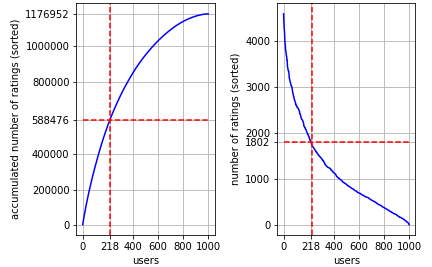
\includegraphics[width=0.45\textwidth]{histo}
      \caption{Determining number of ratings for split on support}
      \label{fig:histo}
    \end{figure}

    Then we use the same features as previously and apply Ridge Regression to each of the two sets separately, obtaining different weights for the ratings depending on whether they have a \emph{low} or \emph{high} user support.
  % subsection user_support (end)

\section{Results}
\label{sec:results}
  In this section we present the results obtained by applying the prediction models described previously. Although the ratings are meant to be integer values, we did not round our predictions since this increased our RMSE value.
  \subsection{Collaborative Filtering methods} % (fold)
  \label{sub:individual_cf_methods}
    Figure \ref{fig:RMSECF} shows the test errors obtained for each of the collaborative filtering methods we described previously, that were obtained using the same 5 folds that we used for generating the predictions of the \emph{training} dataset.
    The baseline prediction has the highest RMSE, whereas the lowest RMSE is achieved by the SVD method from the Surprise library followed by the matrix factorization by ALS method that we implemented.

    \begin{figure}[htp]
      \centering
      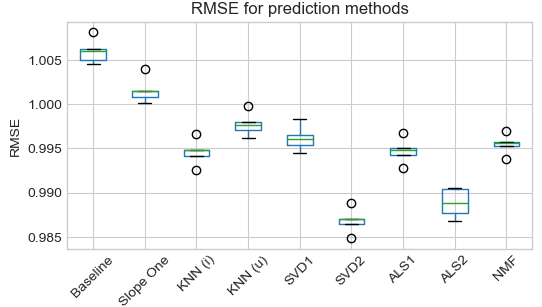
\includegraphics[width=0.45\textwidth]{RMSECF}
      \caption{Test RMSE for CF prediction methods}
      \label{fig:RMSECF}
    \end{figure}


    It is interesting for both this and the upcoming sections to compare how similar the predictions are to each other, especially since this is desirable in order to obtain a better ensemble. Figure \ref{fig:CFcompcorr} shows the Pearson correlation between each pair of prediction methods, and Figure \ref{fig:CFcompmax} shows the maximum difference between predictions.

    \begin{figure}[htp]
      \centering
      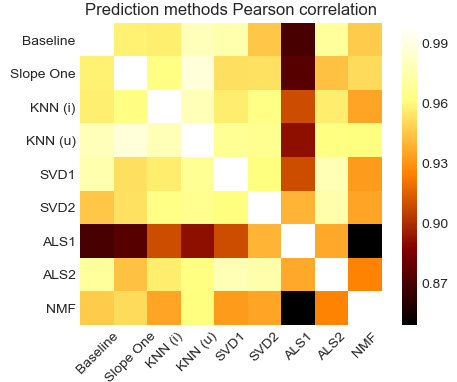
\includegraphics[width=0.35\textwidth]{CFcompcorr}
      \caption{Correlation between predictions} % subcaption
      \label{fig:CFcompcorr}
    \end{figure}

    \begin{figure}[htp]
      \centering
      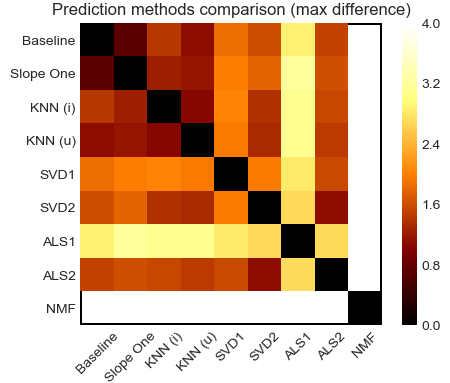
\includegraphics[width=0.35\textwidth]{CFcompmax}
      \caption{Maximum difference between predictions} % subcaption
      \label{fig:CFcompmax}
    \end{figure}

    Although the correlation is high, it can be seen in Figure \ref{fig:CFcompmax} that there are certain ratings for which there are considerable differences across different methods. It is for this reason that we have decided to include all of the predictions obtained with these prediction methods in the ensemble.
  % subsection individual_cf_methods (end)
  \subsection{Ridge Regression ensembling} % (fold)
  \label{sub:ridge_regression_ensembling}
    In order to test the RMSE achieved by the ensemble we decided to split the \emph{training} dataset in 95\% for train and 5\% for test. We then obtained the predictions for the CF models for the train dataset dividing it into 5 disjoint subsets - as we had done previously. We obtained an RMSE of 0.9826 for test with this ensemble.
  % subsection ridge_regression_ensembling (end)
  \subsection{Ensembling splitting by user support} % (fold)
  \label{sub:ensembling_considering_user_support}
    Afterwards we split the ratings into two subsets according to their user support, and apply Ridge Regression to each of them separately.

    The justification for this is shown in Figures \ref{fig:RMSECFH} and \ref{fig:RMSECFL}, which show the RMSE that the CF methods obtain for the ratings depending on their level of support. These figures were obtained by using all the \emph{training} dataset, so they can be compared to Figure \ref{fig:RMSECF} as well.
    \begin{figure}[htp]
      \centering
      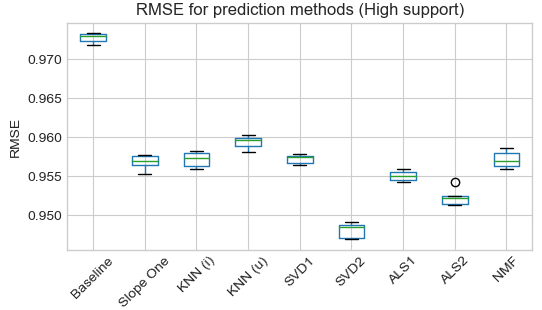
\includegraphics[width=0.45\textwidth]{RMSECFH}
      \caption{Test RMSE for prediction methods (high support)}
      \label{fig:RMSECFH}
    \end{figure}
    \begin{figure}[htp]
      \centering
      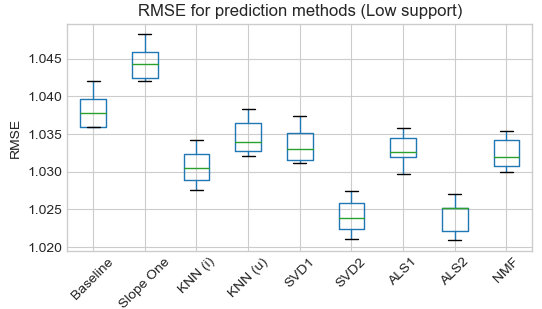
\includegraphics[width=0.45\textwidth]{RMSECFL}
      \caption{Test RMSE for prediction methods (low support)}
      \label{fig:RMSECFL}
    \end{figure}
    It is expected that the error is higher when there are fewer ratings available, but it is particularly interesting to compare how well the models do compared to each other depending on the support.

    We then tested the ensemble considering the same 95\% and 5\% train and test subsets as in the previous ensemble, in this case achieving an RMSE score of 0.9757.
  % subsection ensembling_considering_user_support (end)
\section{Discussion}
\label{sec:discussion}
  Our first approach for improving the predictions was using an ensemble of methods. The best simple predictor was the MF by ALS method that we implemented, that achieved an average RMSE score of 0.9875 for the test data. Ridge Regression applied to the set of features that we created lowered the RMSE to 0.9826.
  Afterwards we lowered the RMSE to 0.9757 by ensembling high and low user support ratings separately.

  Some CF models achieved very different RMSE scores depending on if the ratings had a high or a low user support. For instance, we can look at Baseline and Slope One since when predicting low support ratings the baseline method yields better results than Slope One, as opposed to what we saw in Figure  \ref{fig:RMSECF}. It is likely that Slope One reduced its overall RMSE by improving its predictions for high support ratings, resulting in the baseline method outperforming it for low support data.

  However we did see that the errors achieved by CF methods for low user support were higher than for high support. Although applying Ridge Regression to each group of ratings separately improved the score, it seems that training some models so that they specifically minimize prediction errors for low support ratings could have improved our results. This is a common approach in the literature \cite{jahrer2010combining} and we can consider it as future work.


\section{Summary}
\label{sec:tips-writing}
  We focused on implementing a recommendation system based on ensemble techniques, using Ridge Regression for ensembling. The advantage of this is that we can use individual predictions already obtained with CF methods, and combine them in a relatively simple way.

  We were able to improve the RMSE score of our prediction ensemble by doing feature engineering and using a binned approach.

\bibliographystyle{IEEEtran}
\bibliography{literature}

\end{document}
